\documentclass[11pt]{article}
\usepackage[utf8]{inputenc}
\usepackage[colorlinks]{hyperref}
\usepackage{graphicx}  % For including figures
\usepackage{amsmath}   % For math symbols
\usepackage{amssymb}   % For math symbols
\usepackage{hyperref}  % For clickable links
\usepackage{geometry}  % For setting margins
\usepackage{setspace}  % For setting line spacing
\usepackage{fancyhdr}  % For customizing headers
\usepackage{cite}      % For bibliography
\usepackage{lipsum}    % For placeholder text
\usepackage{titlesec}  % For subsection formatting
\usepackage{booktabs}  % For table lines
\usepackage{tikz}      % For drawing graphs
\usepackage{caption}   % For captions
\usepackage{float}     % For placing figures
\usepackage{subcaption} % For subfigures

\newcommand{\subsubsubsection}[1]{
  \vspace{1em} % Space above the section
  \noindent\textbf{#1} % Bold the section title
  \vspace{0.5em} % Space below the section
}

\geometry{letterpaper, margin=1in}

\setlength{\parindent}{0pt}
\setlength{\parskip}{1em}

\hypersetup{
    linkcolor = {black},
    citecolor = {violet},
    urlcolor = {teal}
}

\title{Efficient and Accurate Triangle Count Estimation in Large Networks}
\date{}
\author{
  \textbf{Sophia Hubscher}\\
  Robert and Donna Manning College of Information and Computer Sciences\\
  University of Massachusetts Amherst\\
  \texttt{shubscher@umass.edu}\\
}

\begin{document}

\maketitle

\vfill

\noindent\textbf{Committee Chair: }Professor Cameron Musco
\;\;\;\texttt{cmusco@cs.umass.edu} \\
\textbf{Second Committee Member: }Professor Ghazaleh Parvini\;\;\;\texttt{gparvini@cs.umass.edu} \\
\textbf{Research Type: } Thesis \\

\newpage

\begin{abstract}
ABSTRACT HERE
\end{abstract}

\newpage

\tableofcontents

\newpage

\section{Introduction}

Counting triangles is a fundamental problem in graph theory with widespread applications in social networks, bioinformatics, and more \cite{lovasz_large_2012}.
These triangles, are formed by three mutually connected nodes, as shown in Figure~\ref{fig:triangles}, which contains three triangles.
While these triangles appear simple, they are a powerful structural motif that can reveal important insights the networks they are found in.

\begin{figure}[H]
    \centering
    % Create a minipage for the graph
    \begin{minipage}{0.45\textwidth}
        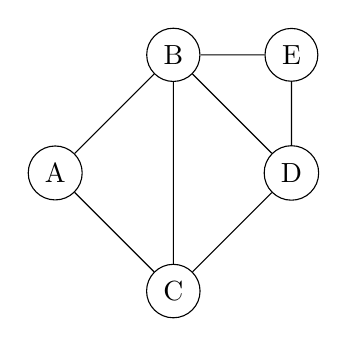
\begin{tikzpicture}[scale=1.5]
            % Define vertices
            \node[circle, draw] (A) at (0, 0) {A};
            \node[circle, draw] (B) at (1, 1) {B};
            \node[circle, draw] (C) at (1, -1) {C};
            \node[circle, draw] (D) at (2, 0) {D};
            \node[circle, draw] (E) at (2, 1) {E};

            % Draw edges to form triangles
            \draw (A) -- (B);
            \draw (A) -- (C);
            \draw (B) -- (C); 
            \draw (B) -- (D);
            \draw (C) -- (D);
            \draw (B) -- (E);
            \draw (D) -- (E);
        \end{tikzpicture}
        \caption{Graph with triangles formed between vertices (A, B, C), (B, C, D) and (B, D, E).}
        \label{fig:triangles}
    \end{minipage}%
\end{figure}

These triangles are more than just theoretical constructs.
In social network graphs, for example, they can represent closed friendships or tightly-knit groups, signaling levels of local connectivity in a network.
This, in turn, can reflect greater patterns and structures within a network.
For example, in social media platforms, triangles are used to model relationships between users, where closed triangles indicate strong communities or mutual interests.
A study analyzing the effect of recommender systems on X (formerly Twitter) demonstrated how an increase in closed triangles following the introduction of a ``Who to Follow'' friend-to-friend recommendation algorithm served as evidence of the algorithm's efficacy \cite{su_effect_2016}.

Additionally, triangles can be used to understand relationships within biological networks.
For example, a study on yeast protein interaction networks used analysis of triangles to find transitive relationships between genes and proteins \cite{ye_commensurate_2005}.
The researchers constructed graphs called ``genetic congruence networks," connecting genes that shared similar interaction partners.
These networks showed a higher-than-expected occurrence of triangles, indicating a strong correlation between genetic congruence and protein interactions.
This suggests that triangles can capture important structural patterns, such as proteins that function within the same biological pathway or complex.
Like in the case of social network analysis, this example illustrates how triangle metrics are not just useful for theoretical analysis but also for practical applications.

While the utility of triangle-based metrics is well-documented, counting triangles efficiently in large graphs remains computationally challenging.
Direct enumeration methods involve inspecting all possible triples of nodes in the graph, a process with a worst-case time complexity of $O(n^3)$ where $n$ is the number of nodes \cite{al_hasan_triangle_2018}.
On smaller networks, this runtime may not pose issues, but unfortunately, for large graphs, especially sparse ones, where the number of edges is much smaller compared to the number of possible edges (as illustrated in Figures \ref{fig:dense_graph} and \ref{fig:sparse_graph}), efficiently counting these triangles poses significant computational challenges.

As graphs grow larger and more complex, direct methods for counting triangles become increasingly time-consuming, making it difficult to handle graphs of practical size in real-world applications.
This issue is particularly relevant in the era of big data, where networks of millions or even billions of nodes and edges are common, and computational efficiency is critical.

\begin{figure}[H]
    \centering
    \begin{minipage}{0.45\textwidth}
        \centering
        % Dense graph
        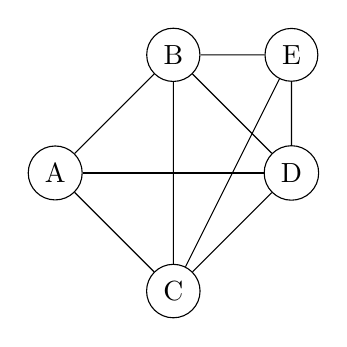
\begin{tikzpicture}[scale=1.5]
            % Define vertices
            \node[circle, draw] (A) at (0, 0) {A};
            \node[circle, draw] (B) at (1, 1) {B};
            \node[circle, draw] (C) at (1, -1) {C};
            \node[circle, draw] (D) at (2, 0) {D};
            \node[circle, draw] (E) at (2, 1) {E};
            % Draw edges to form a dense graph
            \draw (A) -- (B);
            \draw (A) -- (C);
            \draw (A) -- (D);
            \draw (B) -- (C);
            \draw (B) -- (D);
            \draw (B) -- (E);
            \draw (C) -- (D);
            \draw (C) -- (E);
            \draw (D) -- (E);
        \end{tikzpicture}
        \caption{Dense Graph with many edges relative to the number of nodes.}
        \label{fig:dense_graph}
    \end{minipage}%
    \hspace{0.5cm}
    \begin{minipage}{0.45\textwidth}
        \centering
        % Sparse graph
        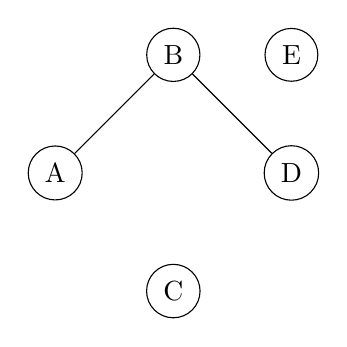
\begin{tikzpicture}[scale=1.5]
            % Define vertices
            \node[circle, draw] (A) at (0, 0) {A};
            \node[circle, draw] (B) at (1, 1) {B};
            \node[circle, draw] (C) at (1, -1) {C};
            \node[circle, draw] (D) at (2, 0) {D};
            \node[circle, draw] (E) at (2, 1) {E};
            % Draw edges to form a sparse graph
            \draw (A) -- (B);
            \draw (B) -- (D);
        \end{tikzpicture}
        \caption{Sparse Graph with few edges relative to the number of nodes.}
        \label{fig:sparse_graph}
    \end{minipage}
\end{figure}

To address these challenges, researchers have developed a variety of approaches to count triangles efficiently.
Some deterministic methods outlined in more detail in the background section of this proposal decrease the time it takes to compute global triangle counts \cite{strassen_gaussian_1969}.
However, these methods still face scalability issues.
As a result, randomized algorithms \cite{tsourakakis_doulion_2009, seshadhri_triadic_2013, tsourakakis_fast_2008} have emerged as a promising alternative.
By leveraging probabilistic techniques, these algorithms provide approximate triangle counts with significant reductions in runtime while maintaining a high degree of accuracy.

Thus, this thesis aims to use randomized algorithms to find new, fast, accurate ways to estimate triangle counts that can be used in real-world applications.

\newpage

\section{Notation}

\begin{table}[ht]
    \centering
    \caption{List of notation used.}
    \begin{tabular}{ll}
        \toprule
        \textbf{Symbol} & \textbf{Description} \\
        \midrule
        $G(V, E)$       & Graph with $V$ vertices and $E$ edges. \\
        $n = |V|$       & Number of vertices in graph $G$. \\
        $m = |E|$       & Number of edges in graph $G$. \\
        $A$             & The adjacency matrix for the graph $G$. \\
        $\Delta_i$      & Number of triangles node $i$ participates in. \\
        $\Delta$        & Total number of triangles in $G$. \\
        $d_i$           & Degree of node $i$. \\
        \bottomrule
    \end{tabular}
    \label{tab:notation}
\end{table}

\newpage

\section{Background}

\subsection{Types of Graphs}

In graph theory, graphs are classified as either directed or undirected.  
An \emph{undirected graph} is one in which edges have no specific direction, so the relationship between connected nodes is mutual: If $u$ connects to $v$, then $v$ connects to $u$.  
In contrast, a \emph{directed graph}, or digraph, has edges with a defined direction—$u$ may point to $v$ without $v$ pointing to $u$.  
This directional property is particularly relevant when calculating triangle counts, as a triangle in a directed graph can follow a specific directional sequence.  
In this discussion, we generally refer to undirected graphs unless otherwise specified, although the methods described can be extended to directed graphs as well.

\subsection{Methods for Triangle Counting}

Triangle counting can be approached in a variety of ways, each with its own advantages and disadvantages. 
One of the simplest methods is the brute force technique, where all distinct sets of three vertices ${u, v, w}$ are enumerated and checked for the existence of a triangle.
This involves examining every possible combination of vertices in the graph and testing whether all three edges $(u, v)$, $(v, w)$, and $(w, u)$ exist. 

Assuming optimal conditions with edges stored in a hash table, where edge retrieval takes $O(1)$ time, the time complexity of this brute force approach is $\Theta(n^3)$. 
This complexity stems from the fact that ${n \choose k} = \Theta(n^k)$, and thus, ${n \choose 3} = \Theta(n^3)$ \cite{al_hasan_triangle_2018}. 

While this method is straightforward, it is inefficient for large graphs due to its high computational cost.
Additionally, this method is no more efficient on sparse graphs (those with relatively few edges compared to the maximum number of edges possible) than on dense ones, which is another area for improvement.
Thus, researchers have turned to alternative triangle counting and estimation methods.

\subsubsection{Sampling Methods}

One of the most effective ways to estimate triangle counts in large, sparse graphs is through sampling methods.
These methods rely on randomly selecting edges or vertices and then inspecting their local neighborhoods for the presence of triangles.
Sampling-based techniques are particularly useful in scenarios where calculating the exact triangle count is computationally expensive or unnecessary.

Additionally, sampling algorithms often provide tunable accuracy, allowing for a trade-off between precision and performance, making them ideal for processing large-scale networks.

\subsubsubsection{Edge Sampling}

In edge sampling, we randomly sample a subset of edges from the graph, count the number of triangles in the subgraph, and scale up to reach our estimate.

One key edge sampling algorithm is Doulion \cite{tsourakakis_doulion_2009}, in which each edge in our graph $G$ is sampled with probability $p$.
As all triangles consist of three edges, this means that all triangles in $G$ have probability $p^3$ of being counted.
Thus, the number of triangles counted is scaled by $\frac{1}{p^3}$ to achieve a final estimate.

Other algorithms extend this even further.
For example, a parallel implementation of Doulion \cite{arifuzzaman_parallel_2012}, where each processor independently sparsifies its assigned partition of the graph, can improve accuracy.

In all of these algorithms though, the key piece of their efficiency and efficacy is the sampling of edges to get a good picture of the graph's structure without counting every triangle individually.

\subsubsubsection{Wedge Sampling}

Wedge sampling \cite{seshadhri_triadic_2013} focuses on estimating wedges—triplets of nodes that form two edges but not necessarily a triangle.
A wedge is defined by three vertices $(u, v, w)$ where $u$ is adjacent to both $v$ and $w$, but $v$ and $w$ may or may not be adjacent (see Figure~\ref{fig:wedge_diagram}).

\begin{figure}[h]
    \centering
    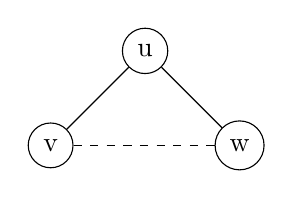
\begin{tikzpicture}[scale = 1.2]
        % Nodes
        \node[circle, draw] (u) at (0,1) {u};
        \node[circle, draw] (v) at (-1,0) {v};
        \node[circle, draw] (w) at (1,0) {w};

        % Edges
        \draw[-] (u) -- (v);
        \draw[-] (u) -- (w);

        % Dashed line to indicate possible or absent connection
        \draw[dashed] (v) -- (w);
    \end{tikzpicture}
    \caption{Wedge formed by vertices $u$, $v$, and $w$. Nodes $v$ and $w$ may or may not be connected.}
    \label{fig:wedge_diagram}
\end{figure}

First, the algorithm counts the total number of wedges in the graph.
To count these wedges, only one pass over all nodes is required, as at each node, every unique pair of outgoing edges from the node is counted as a single wedge.
Thus, this operation takes $O(m)$ time where $m$ is the number of edges in $G$.

Once wedges are sampled, the algorithm checks how many of them are closed (i.e., form triangles).
The number of triangles can then be estimated by multiplying the number of total wedges by the fraction of all wedges that were closed in the sample.
Wedge sampling tends to work well in graphs with a large number of high-degree vertices, where it becomes easier to sample many wedges at once, but unlike edge sampling, it cannot be efficiently done using data structures like adjacency matrices or adjacency lists.
Thus, wedge sampling comes with an additional preprocessing step that adds to runtime.

\subsubsection{Linear Algebraic Methods}

Along with sampling, we can employ linear algebraic techniques to increase the speed of our triangle counting.

Graphs can be conveniently represented using adjacency matrices, which, in social network analysis, are typically referred to as \emph{sociomatrices} \cite{beum_method_1950}. 
In these matrices, each row and column represents a node, and edges between nodes are represented as 1s in the corresponding matrix entry.

\begin{figure}[H]
    \centering
    % Create a minipage for the graph
    \begin{minipage}{0.45\textwidth}
        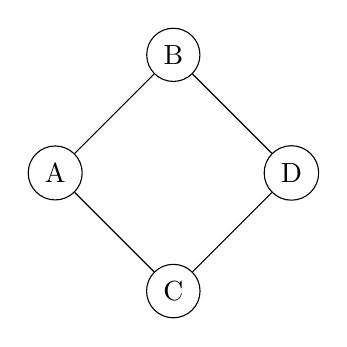
\begin{tikzpicture}[scale=1.5]
            % Define vertices
            \node[circle, draw] (A) at (0, 0) {A};
            \node[circle, draw] (B) at (1, 1) {B};
            \node[circle, draw] (C) at (1, -1) {C};
            \node[circle, draw] (D) at (2, 0) {D};

            % Draw edges
            \draw (A) -- (B);
            \draw (A) -- (C);
            \draw (B) -- (D);
            \draw (C) -- (D);
        \end{tikzpicture}
        \caption{Graph representation of vertices A, B, C, and D.}
    \end{minipage}%
    \hfill
    % Create a minipage for the adjacency matrix
    \begin{minipage}{0.45\textwidth}
        \[
        A =
        \begin{bmatrix}
        0 & 1 & 1 & 0 \\
        1 & 0 & 0 & 1 \\
        1 & 0 & 0 & 1 \\
        0 & 1 & 1 & 0 \\
        \end{bmatrix}
        \]
        \caption{Adjacency matrix corresponding to the graph.}
    \end{minipage}
\end{figure}

By using these adjacency matrices and leveraging linear algebra techniques, we can calculate triangle counts more efficiently. 
One simple method using the adjacency matrix is to use the following formula where $A$ is the adjacency matrix corresponding to the graph $G$ and $\Delta$ is the global triangle count in $G$:

\[
\Delta = \frac{1}{6} \mathrm{trace}(A^3)
\]

This formula is derived from the fact that the diagonal elements of $A^3$ count the number of length-three paths (i.e. triangles) that each vertex participates in.
Each triangle can be formed from six of these length-three paths, as each triangle can be drawn starting at any of its three nodes and moving either clockwise or counter-clockwise, as illustrated in Figure~\ref{fig:triangle-traversal}.
Thus, the trace of $A^3$ is divided by six to scale down to the global triangle count.

\begin{figure}[H]
    \centering
    % First triangle
    \begin{subfigure}{0.15\textwidth}
        \centering
        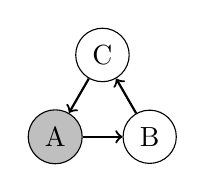
\begin{tikzpicture}[scale=1.2]
            % Define vertices
            \node[circle, draw, fill=gray!50] (A) at (0,0) {A};
            \node[circle, draw] (B) at (1,0) {B};
            \node[circle, draw] (C) at (0.5,0.866) {C};

            % Draw edges with arrows
            \draw[thick, ->] (A) -- (B);
            \draw[thick, ->] (B) -- (C);
            \draw[thick, ->] (C) -- (A);
        \end{tikzpicture}
    \end{subfigure}
    % Second triangle
    \begin{subfigure}{0.15\textwidth}
        \centering
        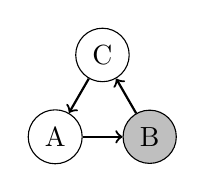
\begin{tikzpicture}[scale=1.2]
            % Define vertices
            \node[circle, draw, fill=gray!50] (B) at (1,0) {B};
            \node[circle, draw] (C) at (0.5,0.866) {C};
            \node[circle, draw] (A) at (0,0) {A};

            % Draw edges with arrows
            \draw[thick, ->] (B) -- (C);
            \draw[thick, ->] (C) -- (A);
            \draw[thick, ->] (A) -- (B);
        \end{tikzpicture}
    \end{subfigure}
    % Third triangle
    \begin{subfigure}{0.15\textwidth}
        \centering
        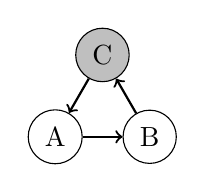
\begin{tikzpicture}[scale=1.2]
            % Define vertices
            \node[circle, draw, fill=gray!50] (C) at (0.5,0.866) {C};
            \node[circle, draw] (A) at (0,0) {A};
            \node[circle, draw] (B) at (1,0) {B};

            % Draw edges with arrows
            \draw[thick, ->] (C) -- (A);
            \draw[thick, ->] (A) -- (B);
            \draw[thick, ->] (B) -- (C);
        \end{tikzpicture}
    \end{subfigure}
    % Fourth triangle
    \begin{subfigure}{0.15\textwidth}
        \centering
        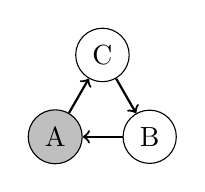
\begin{tikzpicture}[scale=1.2]
            % Define vertices
            \node[circle, draw, fill=gray!50] (A) at (0,0) {A};
            \node[circle, draw] (C) at (0.5,0.866) {C};
            \node[circle, draw] (B) at (1,0) {B};

            % Draw edges with arrows
            \draw[thick, ->] (A) -- (C);
            \draw[thick, ->] (C) -- (B);
            \draw[thick, ->] (B) -- (A);
        \end{tikzpicture}
    \end{subfigure}
    % Fifth triangle
    \begin{subfigure}{0.15\textwidth}
        \centering
        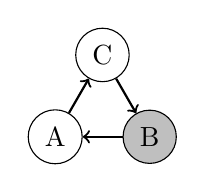
\begin{tikzpicture}[scale=1.2]
            % Define vertices
            \node[circle, draw, fill=gray!50] (B) at (1,0) {B};
            \node[circle, draw] (A) at (0,0) {A};
            \node[circle, draw] (C) at (0.5,0.866) {C};

            % Draw edges with arrows
            \draw[thick, ->] (B) -- (A);
            \draw[thick, ->] (A) -- (C);
            \draw[thick, ->] (C) -- (B);
        \end{tikzpicture}
    \end{subfigure}
    % Sixth triangle
    \begin{subfigure}{0.15\textwidth}
        \centering
        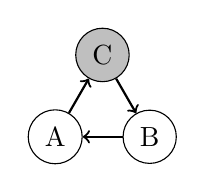
\begin{tikzpicture}[scale=1.2]
            % Define vertices
            \node[circle, draw, fill=gray!50] (C) at (0.5,0.866) {C};
            \node[circle, draw] (B) at (1,0) {B};
            \node[circle, draw] (A) at (0,0) {A};

            % Draw edges with arrows
            \draw[thick, ->] (C) -- (B);
            \draw[thick, ->] (B) -- (A);
            \draw[thick, ->] (A) -- (C);
        \end{tikzpicture}
    \end{subfigure}
    \caption{Six different ways to arrive at a length-three path in a triangle.}
    \label{fig:triangle-traversal}
\end{figure}

To compute $A^3$, we first need to calculate $A^2$ (which takes $O(n^3)$ for an $n \times n$ matrix, $n$ thus also being the number of nodes in our graph $G$) and then multiply $A^2$ by $A$ (also $O(n^3)$).
Thus, the total complexity for computing $A^3$ is $O(n^3)$.
After computing $A^3$, calculating the trace takes $O(n)$, as we need to iterate over the $n$ diagonal elements.
Thus, the overall runtime complexity for the operation is $O(n^3)$.
While this is not a direct improvement over the runtime of the naive algorithm, this strategy forms the basis of many faster methods.

\subsubsubsection{Strassen's Algorithm}

This runtime analysis above assumes that matrix multiplication is performed using the standard algorithm.
However, more sophisticated techniques, such as Strassen's algorithm \cite{strassen_gaussian_1969}, can reduce matrix multiplication time.
In this algorithm, that is used on large, square matrices, such as undirected sociomatrices, each matrix is divided into smaller submatrices on which a series additions and multiplications are performed.

Specifically, Strassen's algorithm reduces the complexity of multiplying two $n \times n$ matrices to approximately $O(n^{\log_2 7})$, which is about $O(n^{2.81})$.
Computing $A^2$ using Strassen's algorithm will take $O(n^{\log_2 7})$.
Then, multiplying $A^2$ by $A$ again takes $O(n^{\log_2 7})$.
Therefore, the total complexity for computing $A^3$ with Strassen's algorithm is $O(n^{\log_2 7}) + O(n^{\log_2 7}) = O(n^{\log_2 7})$, or roughly $O(n^{2.81})$.

To contextualize this, on a $2 \times 2$ matrix, the $n^3$ multiplications required for the naive method would mean we would complete $2^3 = 8$ multiplications.
With Strassen's method and its $n^{\log_2 7}$ multiplications, there would instead only be $2^{\log_2 7} = 7$ multiplications computed.
On larger matrices, this leads to a significant speedup.

There are matrix multiplication algorithms that are even faster, such as one with a $O(n^{2.371552})$ runtime, but this algorithm relies on the use of extremely large constants and is thus rarely used in real-world applications \cite{williams_new_2023}.

\subsubsubsection{EigenTriangle Algorithm}

Another significant approach in triangle counting is the use of spectral methods.
One such method is the EigenTriangle algorithm \cite{tsourakakis_fast_2008}, which estimates the triangle count $\Delta$ by considering the spectral decomposition of the adjacency matrix $A$.

The EigenTriangle algorithm is based on the observation that the number of triangles in a graph is closely related to the spectrum of its adjacency matrix.
In particular, the adjacency matrix $A$ is decomposed as:

\[
A = U \Lambda U^T,
\]

where $U$ is a matrix whose columns are the eigenvectors of $A$, and $\Lambda$ is a diagonal matrix containing the corresponding eigenvalues.

Once the decomposition is performed, the number of triangles can be computed exactly using $\Delta = \frac{1}{6} \sum_{i=1}^{n} \lambda_i^3$, and can be estimated using:

\[
\Delta \approx \frac{1}{6} \sum_{i=1}^{k} \lambda_i^3,
\]

where $\lambda_i$ are the $k$ eigenvalues of largest magnitude of the adjacency matrix $A$.
The runtime of EigenTriangle is dominated by the cost of approximating the top $k$ eigenvalues and eigenvectors of $A$, which, using the Lanszos method \cite{cullum_lanczos_2002}, can be done in roughly $O(k m)$ time, where $m$ is the number of edges and $k$ is typically much smaller than the number of nodes $n$.
This is a significant improvement over the runtimes of direct methods.

Specifically, for the direct method in which was compute the trace of $A^3$, we know ${trace}(A^3) = \sum_{i = 1}^{n} \lambda_i(A^3) = \sum_{i = 1}^{n} \lambda_i^3$.
Thus, we see that EigenTriangle approximates ${trace}(A^3)$.
Given this, it makes sense that this runtime is a substantial improvement over the complexity of computing $\mathrm{trace}(A^3)$ directly.

\subsubsubsection{TraceTriangle Algorithm}

The TraceTriangle algorithm \cite{avron_counting_2010} is a randomized algorithm designed for efficient triangle estimation in large graphs.
It leverages trace-based techniques, which compute the trace of matrix powers to approximate the number of triangles.
Specifically, the algorithm relies on the previously mentioned property: $\Delta = \frac{1}{6} \mathrm{trace}(A^3)$, where $A$ is the adjacency matrix of the graph and $\Delta$ is the number of triangles.
However, rather than computing the full matrix multiplication $A^3$, which is computationally expensive for large graphs, the TraceTriangle algorithm uses a randomized approach to approximate this trace, significantly reducing computation time.

This randomized approach is based on Hutchinson's method \cite{hutchinson_stochastic_1990}, which is a technique for estimating the trace of a matrix by randomly sampling vectors.
In this case, this significantly reduces computation time by approximating $\mathrm{trace}(A^3)$ through randomized sampling rather than explicit computation.

The TraceTriangle algorithm is a sampling algorithm, and thus, it's runtime depends on the desired accuracy of output, as more or fewer samples can be taken depending on the application.
Generally though, experiments demonstrate that typically $O(log^2|n|)$, where $n$ is the number of vertices in $G$, samples are required to get good approximations on real-world graphs, and regardless of application, the runtime for taking each sample is $O(|m|)$, where $m$ is the number of edges in $G$.

Comparing TraceTriangle to the EigenTriangle algorithm, TraceTriangle achieves higher accuracy across multiple types of graphs \cite{avron_counting_2010}.
Despite this accuracy advantage, EigenTriangle tends to run more quickly than TraceTriangle on large graphs.
That said, one advantage of TraceTriangle is its potential for parallelization.
This allows TraceTriangle to scale effectively with the size of the graph, ultimately reducing the speed advantage of EigenTriangle in larger computations.

\subsection{General Algorithmic Strategies}

Beyond specific algorithms for triangle counting, various general techniques from theoretical computer science have been adapted for this problem, particularly in designing faster algorithms.

\subsubsection{Variance Reduction}

Variance reduction \cite{prescott_monte_1965} is another general technique that can be applied to triangle estimation, improving accuracy without increasing the number of samples needed.

Variance reduction methods aim to reduce the spread (or variance) of estimations, leading to more reliable results even with fewer samples.
This is particularly important in large-scale graphs, where taking a high number of samples may be computationally infeasible.

In terms of triangle counting, this method can be applied by finding a fast way of estimating the global triangle count, and then using sampling to estimate the error on that count.
Specifically, we can begin by finding a relationship between the degree of nodes and the number of triangles they are involved in.
This can be done by plotting nodes' degrees ($d_i$) versus triangle counts $(\Delta_i)$ on a log-log plot, finding a line of best fit, and then exponentiating as follows:

\[
\log(\Delta_i) \approx \alpha \cdot \log(d_i) + \beta
\]
\[
\Delta_i \approx d_i^\alpha \cdot e^\beta = m_i.
\]

Now, using this equation, we can estimate the overall triangle count $M$ by applying this line of best fit relationship to all nodes in the graph:

\[
M = \sum_{i = 1}^{n} m_i.
\]

Next, we sample our graph to get $s$ nodes, with $s$ being our sample size. For each of these $s$ sampled nodes, we count the number of triangles they are involved in (written $\Delta_i$) and find the difference between those actual triangle counts and their estimated triangle counts using the line of best fit relationship. We then take the sum of these errors and scale them up to estimate the error on our global triangle count (written $E$). Mathematically, this can be expressed as follows:

\[
E = \left( \sum_{i = 1}^{s} \Delta_i - m_i \right) \cdot \frac{n}{s}.
\]

Lastly, we take the sum of our estimate and our error, and divide this sum by three to avoid triple-counting triangles, as each triangle has three nodes it is involved in:

\[
\Delta \approx \frac{M + E}{3}.
\]

Thus, by applying this variance reduction technique, we arrive at an estimate for the triangle count $\Delta$.

\subsubsubsection{Importance Sampling}

One example of a variance reduction method is importance sampling.
When estimating a metric relating to a large population using uniform sampling, where all edges/nodes/wedges/etc. are sampled with the same probability, often a very large number of samples is required to ensure a good relative approximation \cite{lovasz_large_2012}.
This is because uniform sampling does not prioritize areas of the graph that may have a disproportionately large impact on the estimate.
Consequently, the computational cost can be high for achieving a desired accuracy level in many cases.

When using importance sampling \cite{motwani_randomized_1995}, the process is improved by sampling higher-interest nodes with higher probability, focusing computational effort on the most ``important" parts of a graph.
The key idea behind importance sampling is to bias the sampling distribution towards more informative areas of the graph.
For instance, in a graph where certain nodes are highly connected or play a critical role in the overall structure, importance sampling would prioritize these nodes to reduce the variance of the estimates.

Importance sampling can also be applied to triangle counts.
For example, we can prioritize high-degree nodes as the most ``important.''
The weight of this importance is decided by some power $\alpha$ greater than 1 (which is equivalent to uniform sampling).
This $\alpha$ can be tuned to indicate different strengths of relationships between the degree and triangle counts of nodes. 

Once $\alpha$ has been selected, we use it to ascribe each node a probability $p_i$ to each node based in its degree $d_i$:

\[
D = \sum_{i = 1}^{n} d_i^\alpha
\]
\[
p_i = \frac{d_i^\alpha}{D}.
\]

Next, we sample $s$ nodes based on their probabilities $p_i$.
For example if $p_1 = 0.01$ and $p_2 = 0.1$, we are 10 times more likely to sample node 2 than node 1.

Next, for each sampled node we count the number of triangles it is a part of, and then scale that count by $\frac{1}{s \cdot p_i}$.
The sum of all these counts, scaled down by three (as to avoid triple-counting triangles), is our estimate for the global triangle count $\Delta$.

\subsubsection{Learning-Augmented Algorithms}

A learning-augmented algorithm \cite{roughgarden_algorithms_2020} is an algorithm that uses a prediction to boost its performance.
Whereas most algorithms take only the problem their input, learning-augmented algorithms also accept an extra piece of information—usually a prediction about some part of the solution.
The algorithm then uses this prediction to run faster or produce better results.

An example of a learning-augmented algorithm is its use in the maximum weight matching problem.
The maximum weight matching problem \cite{duan_linear-time_2014} is the problem of finding a matching in which the sum of weights is maximized in a weighted graph.
The typical solution for this problem, the Hungarian algorithm, runs in $O(m\sqrt{n})$ time.

When a learning-augmented approach \cite{dinitz_faster_2021} is applied however, where machine-learned predictions are used to ``warm-start" the algorithm, that runtime is significantly reduced when the predictions are accurate.
When the predictions are inaccurate, the runtime is simply the same as in the Hungarian algorithm.

This technique can be applied to triangle counting too.
For example, Tonic \cite{boldrin_fast_2024}, a learning-augmented algorithm for counting triangles in graph streams, leverages predictions about edge ``heaviness" (i.e., the number of triangles they are involved in) to improve the accuracy and speed of triangle counting.
Tonic combines these predictions with sampling methods to keep track of the most relevant edges.
This allows the algorithm to focus on the edges that are most likely to contribute to the triangle count.

Notably, Tonic provides unbiased estimates of triangle counts regardless of the accuracy of the predictor.
However, when the predictor provides useful information on heavy edges, the algorithm produces estimates with reduced variance compared to state-of-the-art alternatives.

In general, this method can be highly effective, as accurate predictions can significantly enhance algorithms' efficiency or result quality.

\newpage

\section{Methods}

\textbf{THIS SECTION HAS NOT BEEN CHANGED SINCE THE PROPOSAL -- WILL BE EDITED}

To evaluate different triangle count estimation methods, I will implement them in Python and then compare their accuracies, runtimes, and sample sizes on different networks.
The first methods implemented will be uniform sampling, importance sampling, variance reduction, and hybrids between these, but as the methods are evaluated, more are likely to arise.
These methods will be applied to a range of synthetic networks and real-world networks from the \href{https://snap.stanford.edu/index.html}{Stanford Network Analysis Platform (SNAP) library}, which includes graphs of different sizes, densities, and structural properties.

\subsection{Datasets}

The datasets used will consist of synthetic networks and real-world graphs from the SNAP library, encompassing diverse domains such as social networks, collaboration networks, and citation networks.
Examples of real-world networks include:

\begin{itemize}
    \item Social Networks: Networks representing friendships on Facebook.
    \item Collaboration Networks: Co-authorship graphs in scientific publications.
    \item Web Graphs: Directed graphs of hyperlinks between websites.
\end{itemize}

In addition to these real-world networks, synthetic networks such as Barabási–Albert \cite{albert_statistical_2002} and Watts-Strogatz \cite{watts_collective_1998} graphs will be generated using the \href{https://networkx.org/}{NetworkX library}.

The synthetic networks will serve as controlled environments for testing the scalability and accuracy of the methods under varying structural parameters.
For instance, Barabási–Albert graphs, which simulate preferential attachment, are used to model networks with power-law degree distributions, while Watts–Strogatz graphs capture small-world properties with tunable clustering and path lengths.
These properties allow for targeted testing of the estimation methods under different conditions.

The datasets used will vary in size, edge density (sparse and dense graphs), and clustering characteristics.
This diversity will highlight the strengths and limitations of each method for triangle count estimation.

For all of these datasets, ground-truth triangle counts will be computed using exact algorithms and compared against the approximate counts from the estimation methods tested.
Using this, we can compare accuracy to metrics such as runtime and sample size.

\subsection{Methods Evaluated}

The initial methods evaluated are all outlined in the literature review above.
As these strategies are evaluated, the most effective will be selected and used in hybrid methods.

\textbf{Uniform Sampling:}
This baseline method involves randomly sampling edges or nodes and scaling up the observed triangle counts proportionally.
While simple, uniform sampling may struggle in graphs with skewed degree distributions.

\textbf{Importance Sampling:}
Edges or nodes more likely to form triangles are prioritized using properties such as degree.
This method aims for higher accuracy with fewer samples, though determining optimal weights is a challenge.

\textbf{Variance Reduction:}
The primary goal of variance reduction techniques are to minimize variability in estimates.

\textbf{Hybrid Approaches:}
To combine the strengths of individual techniques, I will explore strategies that combine multiple of the above approaches.

\subsection{Evaluation Metrics}

The methods will be tested on real-world networks, measuring:

\begin{itemize}
    \item Accuracy: Difference between estimated and true triangle counts.
    \item Runtime: Computational time for generating estimates.
    \item Sample size: The number of graph nodes sampled.
    \item Variance: The variability in triangle count estimates across multiple runs of the same method.
\end{itemize}

In addition to these metrics, the general structure of networks will be compared.
For example, I will analyze which methods perform best on sparse versus dense networks and small versus large netowrks.

\subsection{Implementation}

Algorithms will be implemented in Python using NetworkX and SNAP.
Experiments will run on consistent hardware, with multiple trials to ensure reliable comparisons.

\newpage

\section{Variances}

\subsection{Uniform Sampling}

The global triangle count $\Delta$ can be estimated as $\tilde{\Delta}$ using the following formula:

\[
\tilde{\Delta} = \frac{n}{3s} \sum_{i = 1}^{s} \Delta_i,
\]

where $n$ is the number of nodes in our graph $G$, $s$ is our sample size, and $\sum_{i = 1}^{s} \Delta_i$ is the sum of all sampled triangle counts. 
Using this, we can find the variance of $\tilde{\Delta}$ in terms of $n$, $s$, and $\mathrm{Var}(\Delta_i)$.

\[
\begin{aligned}
\mathrm{Var}(\tilde{\Delta}) &= \mathrm{Var} \left( \frac{n}{3s} \sum_{i=1}^{s} \Delta_i \right) \\
&= \frac{n^2}{9s^2} \mathrm{Var} \left( \sum_{i=1}^{s} \Delta_i \right) \\
&= \frac{n^2}{9s^2} \sum_{i=1}^{s} \mathrm{Var}(\Delta_i)
\end{aligned}
\]

Next, we find $\mathrm{Var}(\Delta_i)$.

\[
\mathrm{Var}(\Delta_i) = \mathbb{E}[(\Delta_i - \mathbb{E}[\Delta_i])^2]
\]

\[
\mathbb{E}[\Delta_i] = \frac{1}{n} \Delta_1 + \frac{1}{n} \Delta_2 + \ldots + \frac{1}{n} \Delta_n = \frac{\Delta}{n}
\]

\[
\begin{aligned}
\mathbb{E}[(\Delta_i - \mathbb{E}[\Delta_i])^2] &= \mathbb{E}[(\Delta_i - \frac{\Delta}{n})^2] \\
&= \sum_{i = 1}^{n} \frac{1}{n} (\Delta_i - \frac{\Delta}{n})^2 \\
&= \sum_{i = 1}^{n} \frac{1}{n} (\Delta_i^2 - 2 \Delta_i \frac{\Delta}{n} + \frac{\Delta^2}{n^2}) \\
&= \frac{1}{n} \sum_{i = 1}^{n} \Delta_i^2 - \frac{2}{n} \sum_{i = 1}^{n} \Delta_i \frac{\Delta}{n} + \frac{1}{n} \sum_{i = 1}^{n} \frac{\Delta^2}{n^2} \\
&= \frac{1}{n} \sum_{i = 1}^{n} \Delta_i^2 - \frac{2}{n} \sum_{i = 1}^{n} \Delta_i \frac{\Delta}{n} + \frac{\Delta^2}{n^2} \\
&= \frac{1}{n} \sum_{i = 1}^{n} \Delta_i^2 - \frac{2\Delta^2}{n^2} + \frac{\Delta^2}{n^2} \\
&= \frac{1}{n} \sum_{i = 1}^{n} \Delta_i^2 - \frac{\Delta^2}{n^2}
\end{aligned}
\]

Now, we can plug our value of $\mathrm{Var}(\Delta_i)$ into $\mathrm{Var}(\tilde{\Delta}) = \frac{n^2}{9s^2} \sum_{i=1}^{s} \mathrm{Var}(\Delta_i)$.

\[
\begin{aligned}
\mathrm{Var}(\tilde{\Delta}) &= \frac{n^2}{9s^2} \sum_{i=1}^{s} [\frac{1}{n} \sum_{i = 1}^{n} \Delta_i^2 - \frac{\Delta^2}{n^2}] \\
&= \frac{n^2}{9s^2} s [\frac{1}{n} \sum_{i = 1}^{n} \Delta_i^2 - \frac{\Delta^2}{n^2}] \\
&= \frac{n^2}{9s} [\frac{1}{n} \sum_{i = 1}^{n} \Delta_i^2 - \frac{\Delta^2}{n^2}] \\
&= \frac{n}{9s} [\sum_{i = 1}^{n} \Delta_i^2 - \frac{\Delta^2}{n}] \\
\end{aligned}
\]

\subsection{Variance Reduction}

Take the estimator of $\Delta_i$ to be denoted by $M$ where $M = \sum_{i = 1}^{n} m_i$ and $m_i = \Delta_i + N(0, \sigma^2)$.

\[
\tilde{\Delta} = \sum_{i = 1}^{n} m_i + \frac{n}{s} \sum_{i = 1}^{s} (m_i - \Delta_i)
\]

\[
\begin{aligned}
\mathrm{Var}(\tilde{\Delta}) &= \sum_{i = 1}^{n} \mathrm{Var}(m_i) + \mathrm{Var}(\frac{n}{s} \sum_{i = 1}^{s} (m_i - \Delta_i)) \\
&= \sum_{i = 1}^{n} \mathrm{Var}(m_i) + \frac{n^2}{s^2} \mathrm{Var}(\sum_{i = 1}^{s} (m_i - \Delta_i)) \\
&= \sum_{i = 1}^{n} \mathrm{Var}(m_i) + \frac{n^2}{s^2} \sum_{i = 1}^{s} \mathrm{Var}(m_i - \Delta_i) \\
&= n \sigma^2 + \frac{n^2}{s^2} \sum_{i = 1}^{s} \mathrm{Var}(m_i - \Delta_i) \\
&= n \sigma^2 + \frac{n^2}{s^2} s \sigma^2 \\
&= n \sigma^2 + \frac{n^2}{s} \sigma^2 \\
\end{aligned}
\]

\newpage

\section{Results}

\newpage

\section{Conclusion}

\newpage

\bibliographystyle{plain}
\bibliography{thesis_bib}

\end{document}
